\documentclass{article}
\usepackage{pgfplots}
\pgfplotsset{compat=1.18}

\begin{document}

\begin{figure}[h]
    \centering
    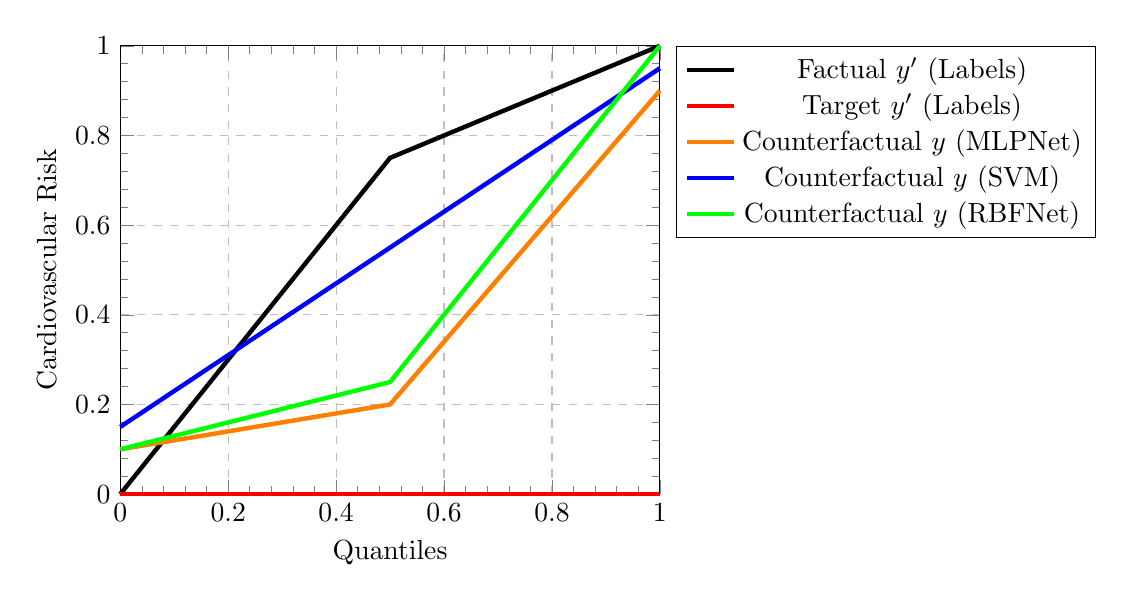
\begin{tikzpicture}
        \begin{axis}[
            xlabel={Quantiles},
            ylabel={Cardiovascular Risk},
            xtick={0, 0.2, 0.4, 0.6, 0.8, 1},
            ytick={0, 0.2, 0.4, 0.6, 0.8, 1},
            legend pos = outer north east,
            ymin=0,
            ymax=1,
            xmin=0,
            xmax=1,
            grid=major,
            grid style=dashed,
            major tick length=5pt,
            minor tick num=4,
            clip=false,
            every axis plot/.append style={ultra thick},
            ]
            
            % Factual y'
            \addplot[black, mark=none] coordinates {(0,0) (0.5,0.75) (1,1)};
            \addlegendentry{Factual $y'$ (Labels)}
            
            % Target y'
            \addplot[red, mark=none] coordinates {(0,0) (0.6,0) (1,0)};
            \addlegendentry{Target $y'$ (Labels)}
            
            % Counterfactual y (MLPNet)
            \addplot[orange, mark=none] coordinates {(0,0.1) (0.5,0.2) (1,0.9)};
            \addlegendentry{Counterfactual $y$ (MLPNet)}
            
            % Counterfactual y (SVM)
            \addplot[blue, mark=none] coordinates {(0,0.15) (0.5,0.55) (1,0.95)};
            \addlegendentry{Counterfactual $y$ (SVM)}
            
            % Counterfactual y (RBFNet)
            \addplot[green, mark=none] coordinates {(0,0.1) (0.5,0.25) (1,1)};
            \addlegendentry{Counterfactual $y$ (RBFNet)}
            
        \end{axis}
    \end{tikzpicture}
    
    \caption{Comparison of factual $y'$, target $y'$, and counterfactual $y$ from different models (MLPNet, SVM, RBFNet). Models are trained on all features, while \gls{dce} optimization is performed only on age, weight, and height.}
    \label{fig:y_label}
\end{figure}

\textit{Description to be supplemented:} [Cardiovascular Disease] The models are trained on all features whereas the \gls{dce} optimization is performed only on age, weight, and height.

\end{document}